\section{Auswertung}
\label{sec:Auswertung}
\paragraph{Justage} 
Nach der Justage der Apparatur wurden folgenden Shimparamter eingestellt.
\begin{equation*}
x = -1,58 \quad y = -6,6 \quad z = 3,68 \quad Z^2 = -1,72	
\end{equation*}
Die Frequenz wurde auf \SI{21,71524}{\mega\Hz} eingestellt. Die Phase auf 
\SI{161}{\degree} einjustiert. Die Periode zwischen den Pulsen wurde 
\SI{11}{\second} gewählt. Für die Messung von $T_2$ und der Diffusionskonstante 
jedoch auf \SI{8}{\second} nachjustiert.

\subsection{Bestimmung der Relaxationszeit \texorpdfstring{$T_1$}{math}}
Zur Messung der Relaxationszeit $T_2$ wurde die induzierte Spannung gegen den variierten 
Pulsabstand $\tau$ gemessen und in Abbildung \ref{fig:T1} aufgetragen. Nach \cite{Anleitung} 
ist der Zusammenhang der beiden Messgrößen gegeben über 
\begin{equation}
U_z = U_0 \cdot \left( 1-2\exp \left( -\frac{\tau}{T_1} \right) \right) + b	\; ,
\end{equation}
dabei bezeichnet $U_z$ die induzierte Spannung. Durch nicht-lineare Ausgleichsrechnung 
ergibt sich $U_0 = \SI{0.667(4)}{\volt}$, $b = \SI{-0.007(4)}{\volt}$ und $T_1 = \SI{2.28(3)}{\second}$. 
\begin{figure}
  \centering
  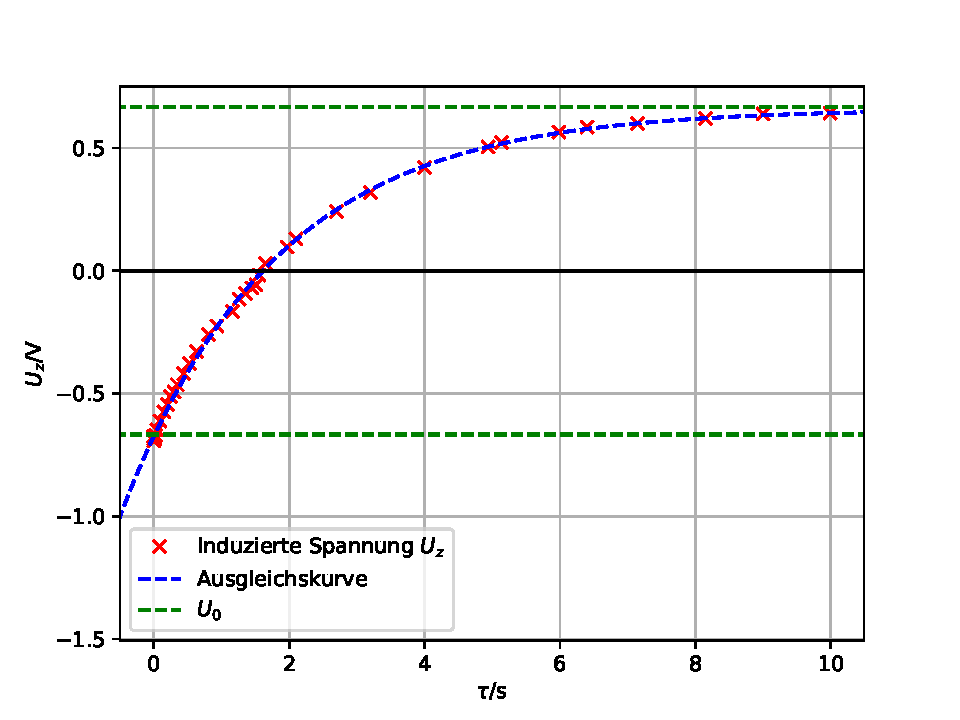
\includegraphics[height = 10cm]{plots/T1plot.pdf}
  \caption{Induzierte Spannung gegen den Pulsabstand aufgetragen.}
  \label{fig:T1}
\end{figure}
\FloatBarrier

\subsection{Bestimmung der Relaxationszeit \texorpdfstring{$T_2$}{math}}
\paragraph{Meiboom-Gill-Methode} Zur Bestimmung der Relaxationszeit $T_2$ wurde mit der Meiboom-Gill-Methode die 
Abbildung des Signals \ref{fig:MGMO} mit einem Oszilloskop erzeugt. Die dazugehörigen Werte wurden ausgelesen und die 
Spitzen des Signals wurden ermittelt. Aus den Werten wurden die Werte ermittelt, die die Einhüllende beschreiben, diese 
wurden logarithmetisiert und in der Abbildung \ref{fig:T2} dargestellt. Zudem wurde mit linearer Ausgleichsrechnung eine 
Ausgleichsgerade berechnet. Der Zusammenhang der Messgrößen ist über die Gleichung \eqref{eq:MYT2} gegeben. Durch 
Anwendung des Logarithmuses ergibt sich für die Ausgleichsgerade
\begin{equation}
\log(U_y) = - \frac{ t + c }{T_2} + \log(U_0)	\; .
\end{equation}
Hierbei bezeichnet $U_y$ die induzierte Spannung, $c$ und $U_0$ sind nur Ausgleichsparamter. 
Damit ergibt sich $c = \SI{0 (5)e-5}{\second}$, $U_0 \approx \SI{609}{\milli\volt}$ und $T_2 = \SI{1.63(6)}{\second}$.
\begin{figure}
  \centering
  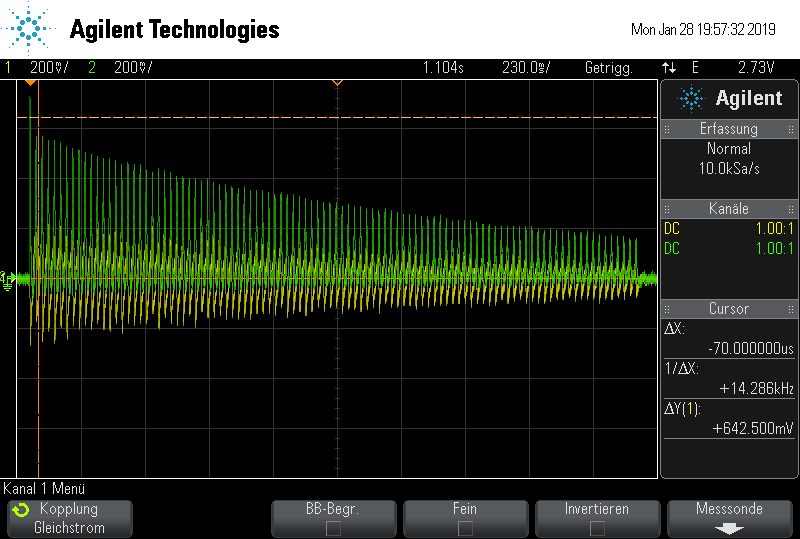
\includegraphics[height = 7cm]{plots/scope_1.png}
  \caption{Abbildung des Meiboom-Gill-Signals auf dem Oszilloskop.}
  \label{fig:MGMO}
\end{figure}
\begin{figure}
  \centering
  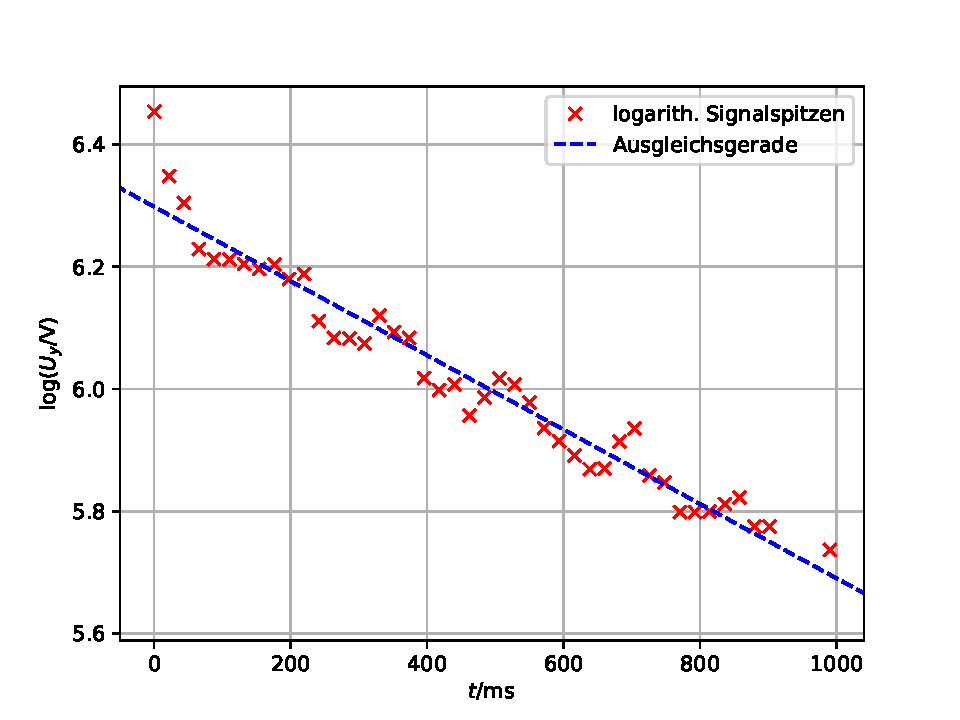
\includegraphics[height = 10cm]{plots/T2plot.pdf}
  \caption{Logarithmitisierte Einhüllende gegen den Pulsabstand.}
  \label{fig:T2}
\end{figure}
\FloatBarrier
\paragraph{Carr-Purcell-Methode}
Desweiteren wurde mit der Carr-Purcell-Methode eine Abbildungen des charakteristischen Signals der Methode mit einem 
Oszilloskop erzeugt, diese ist in der Abbildung \ref{fig:PCM} dargestellt. 
\begin{figure}
  \centering
  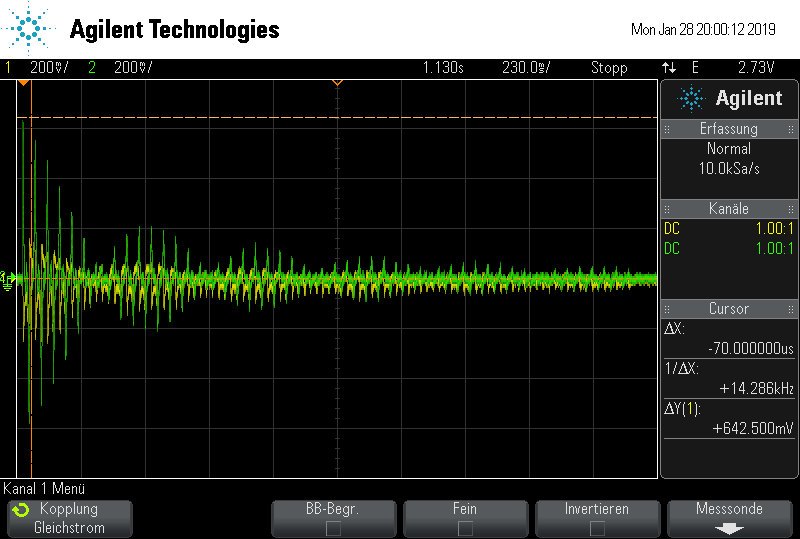
\includegraphics[height = 7cm]{plots/scope_3.png}
  \caption{Abbildung des charakteristischen Carr-Purcell-Signals.}
  \label{fig:PCM}
\end{figure}
\FloatBarrier
\subsection{Bestimmung der Diffusionskonstante}
Für die Messung der Diffusionskonstante $D$ wird die Spannungsamplitude $U_y$ 
gegen die variierte Pulslänge gemessen. Zudem werden 
mit den Cursern des Oszilloskop die Halbwertsbreiten bestimmt. Die Halbwertsbreite sollte bei jeder Messung gleich bleiben, 
weshalb an dieser Stelle nur über die Messwerte gemittelt wurde. Damit ergibt sich die Halbwertsbreite zu 
$t_{\sfrac{1}{2}} =\SI{8(04)e-5}{\second}$. Die Spannungsamplitude wurde logarithmetisiert und gegen die Pulslänge 
aufgetragen. Aus dem Zusammenhang \eqref{eq:DiffusionsBestimmung} folgt eine Ausgleichsgerade der Form
\begin{equation}
\begin{split}
\log(U_y) = - \frac{1}{12}\cdot D \cdot A^2 \cdot t^3 - \frac{t}{T_2} - \log(U_0) \\
\text{mit} \quad t = 2\tau \quad \text{und} \quad 
A = \gamma G = \frac{4 \cdot 2,2}{d \cdot t_{\sfrac{1}{2}}} \quad \text{gegeben über \cite{Anleitung}} \;.
\end{split}
\end{equation}
Dabei bezeichnet $\gamma$ das gyromagnetische Verhältnis, $G$ den Feldgradienten, $d = \SI{4.4}{\milli\meter}$ den 
Probendurchmesser und $U_0$ einen Ausgleichsparamter. Zur Berechnung der Ausgleichkurve wurde der Werte 
für $T_2$ aus dem voran gegangen Kapitel verwendet. Mit linearer Ausgleichsrechnung ergibt sich 
$D= \SI{1.19(5)e-9}{\meter\per\second}$ und $U_0 \approx \SI{0.491}{\volt}$. Der Prozess ist in der Abbildung 
\ref{fig:D} dargestellt. 
\begin{figure}
  \centering
  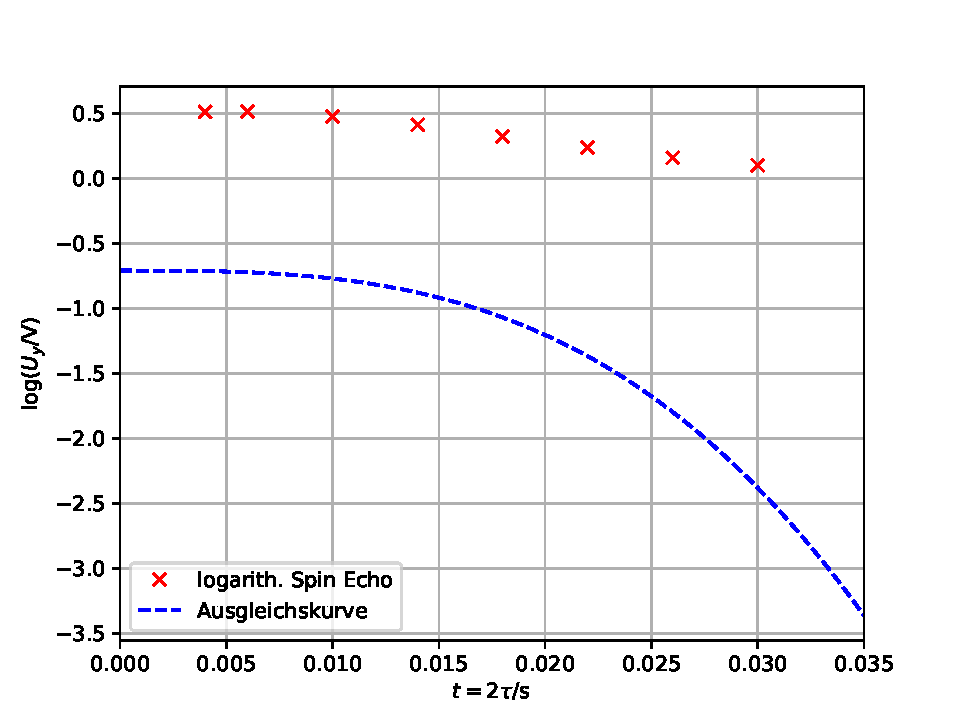
\includegraphics[height = 10cm]{plots/Dplot.pdf}
  \caption{Induzierte Spannung gegen die Pulslänge aufgetragen.}
  \label{fig:D}
\end{figure}
\FloatBarrier
\subsection{Bestimmung der Viskosität}
Zur Bestimmung der Werte muss zuerst $\delta$ bestimmt werden. Dazu wir zwischen den Werten aus Tabelle \ref{tab:VisWerte} 
linear interpoliert. Für die Durchflusszeit $t = \SI{917 .4}{\second}$ folgt $\delta = \SI{0.3(2)}{\second}$. Für die 
Dichte wurde $\rho = \SI{1000}{\kilo\gram\per \cubic\meter}$ angenommen. Dann ergibt sich 
aus der Gleichung \eqref{eq:vis} $\eta = \SI{0.0009391(2)}{\kilo\gram\per\meter\per\second}$.
\subsection{Bestimmung der Molekülradien}
\paragraph{Nach Stokes}
Die Berechnung des Molekülradius nach Stokes ist über die Formel 
\begin{equation}
r = \frac{kT}{6\pi \cdot D \cdot \eta} 	
\end{equation}
nach \cite{Anleitung} gegeben. Für die Temperatur $T$ wurden \SI{20}{\celsius} angenommen. Damit ergibt sich der 
Molekülradius zu $r = \SI{1.92(8)}{\angstrom}$. 
\paragraph{hcp-Kugelpackung}
Bei einer hcp-Kugelpackung wird angenommen, dass \SI{74}{\percent} des Gesamt Volumens eingenommen wird. Daraus folgt 
\begin{gather}
V = \frac{m_{Mol}}{\rho} \\
\implies \frac{4\pi r^3}{3} =\frac{m_{Mol}}{\rho} \\
\implies r_{ges} = \left( \frac{3m_{Mol}}{4\pi \rho } \right)^{\frac{1}{3}} \quad \text{für Gesamtvolumen} \\
\implies r_{hcp} = 0,74 \cdot r_{ges} = \SI{1,42}{\angstrom} \quad \text{für hcp-Packung} \; . 
\end{gather}
Hierbei beschreibt $m_{Mol}$ das Molekülgewicht, bei Wasser gegeben über $m_{Mol} = \SI{16}{\atomicmassunit} + 2\cdot \SI{1}{\atomicmassunit}$
\paragraph{Van-der-Waals-Gas}
Für ein Van-der-Waals-Gas ist das kritische Volumen über die Gleichung 
\begin{equation}
V_{krit}= \frac{3kT_{krit}}{8p_{krit}}	
\end{equation}
gegeben. Daraus folgt 
\begin{equation}
r_{krit} = \left( \frac{9kT_{krit}}{32p_{krit}} \right)^{\frac{1}{3}} = \SI{3,31}{\angstrom} \;.
\end{equation}
Die Gleichugen und Werte dazu wurden aus \cite{spektrum} entnommen.

